\documentclass[a4paper]{article}
\usepackage[a4paper, total={6in, 10in}]{geometry}
% \usepackage{algpseudocode}
\usepackage{float}
\usepackage[english]{babel}
\usepackage[utf8x]{inputenc}
\usepackage{amsmath}
\usepackage{amssymb}
\usepackage{graphicx}
\usepackage[colorinlistoftodos]{todonotes}
\usepackage{algorithm}
%\usepackage{algorithmic}
\usepackage{algpseudocode}
\usepackage{amsmath}
\usepackage{graphics}
\usepackage{epsfig}
% \usepackage[]{algorithm2e}
\usepackage{enumitem}
% \usepackage{enumerate,url}
% \setlength{\parindent}{4em}
% \setlength{\parskip}{2em}
\linespread{1.3}
\title{CS 7646 Manual Strategy Report}
\author{Shu-Ho, CHOU}
\begin{document}
\maketitle
%
% \noindent Please upload:\\
%  1) a PDF cover letter indicating with whom you worked (if applicable), the sources you used, and if you wish, your impressions about the assignment (what was fun, what was difficult, why...); \\
%  2) a PDF with your solutions of Problems 1, 2 and 3; \\
%  3) a PDF of your report for Problem 4; \\
%  4) a single zip file of your code, README, results for Problem 4.\\
%  Each file name should start by \url{<GTusername>_HW1}.
% \\\\
% \noindent Please type your answers in \LaTeX. You may handwrite them if you
% wish, but if we cannot read your handwriting, you will not receive points
% for your answer.
% \\\\
% \noindent Note that MSTs (Problem 4) will be discussed in class on Sept. 5 (see
% course schedule on T-Square).
\section{Indicators}
\subsection{Simple Moving Average}
\begin{itemize}
	\item[(a)] Definition \\
			Simple moving average with window size w days at time t can be defined as \\
			\textbf{SMA[t] = price[t-w:t].mean()} \\
			And the indicator of Simple Moving Average at time t is: \\
			\textbf{indicator\_SMA[t] = $\frac{\text{price[t]}}{\text{SMA[t]}} - 1$}
	\item[(b)] Intuition \\
			The intuition is simple, if the current stock price is higher than the average of past
			few days, then maybe we should expect it to go down, and vice versa. So when
			the indicator has a positive value, we should generally sell, and buy if a
			negative one.
	\item[(c)] Chart and Analysis\\
		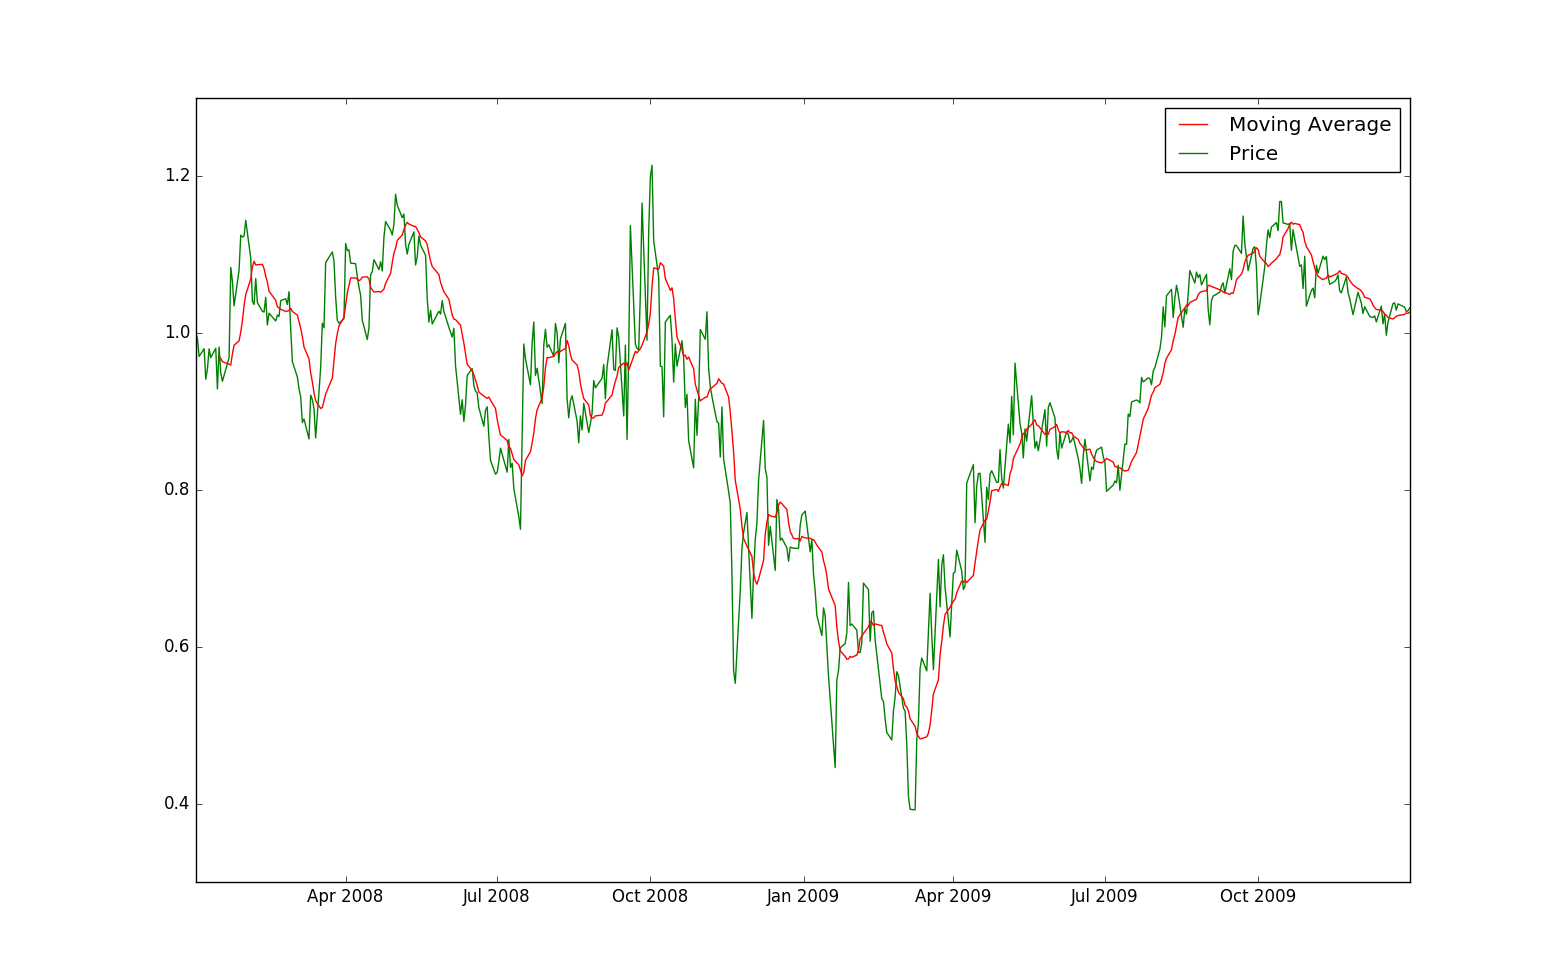
\includegraphics[width=\textwidth]{sma}
			The chart above is generated by window size 10, and we can see that if the value deviates
			a lot from the average, it will finally get back to average generally.


\end{itemize}
\subsection{Bollinger Band}
\begin{itemize}
\item[(a)] Definition \\
		First define STD[t] with window size w as: \\
		\textbf{STD[t] = price[t-w:t].std()} \\
		With the same SMA definition as above mentioned, the indicator of Bollinger Band
		at time t with window size w is: \\
		\textbf{indicator\_BB[t] = $\frac{\text{price[t]-SMA[t]}}{\text{STD[t]}}$}
\item[(b)] Intuition \\
		This is actually similar to SMA, however, Bollinger Band quantitize the deviation
		from moving average by dividing the difference of stock price and moving average by
		the standard deviation of the last few days. It reflects how stable the stock is and
		decide to buy or sell depending on the information. With this indicator, we expect value
		bigger than 1 to be a selling signal, and smaller than -1 to be a buying signal.
\item[(c)] Chart and Analysis\\
	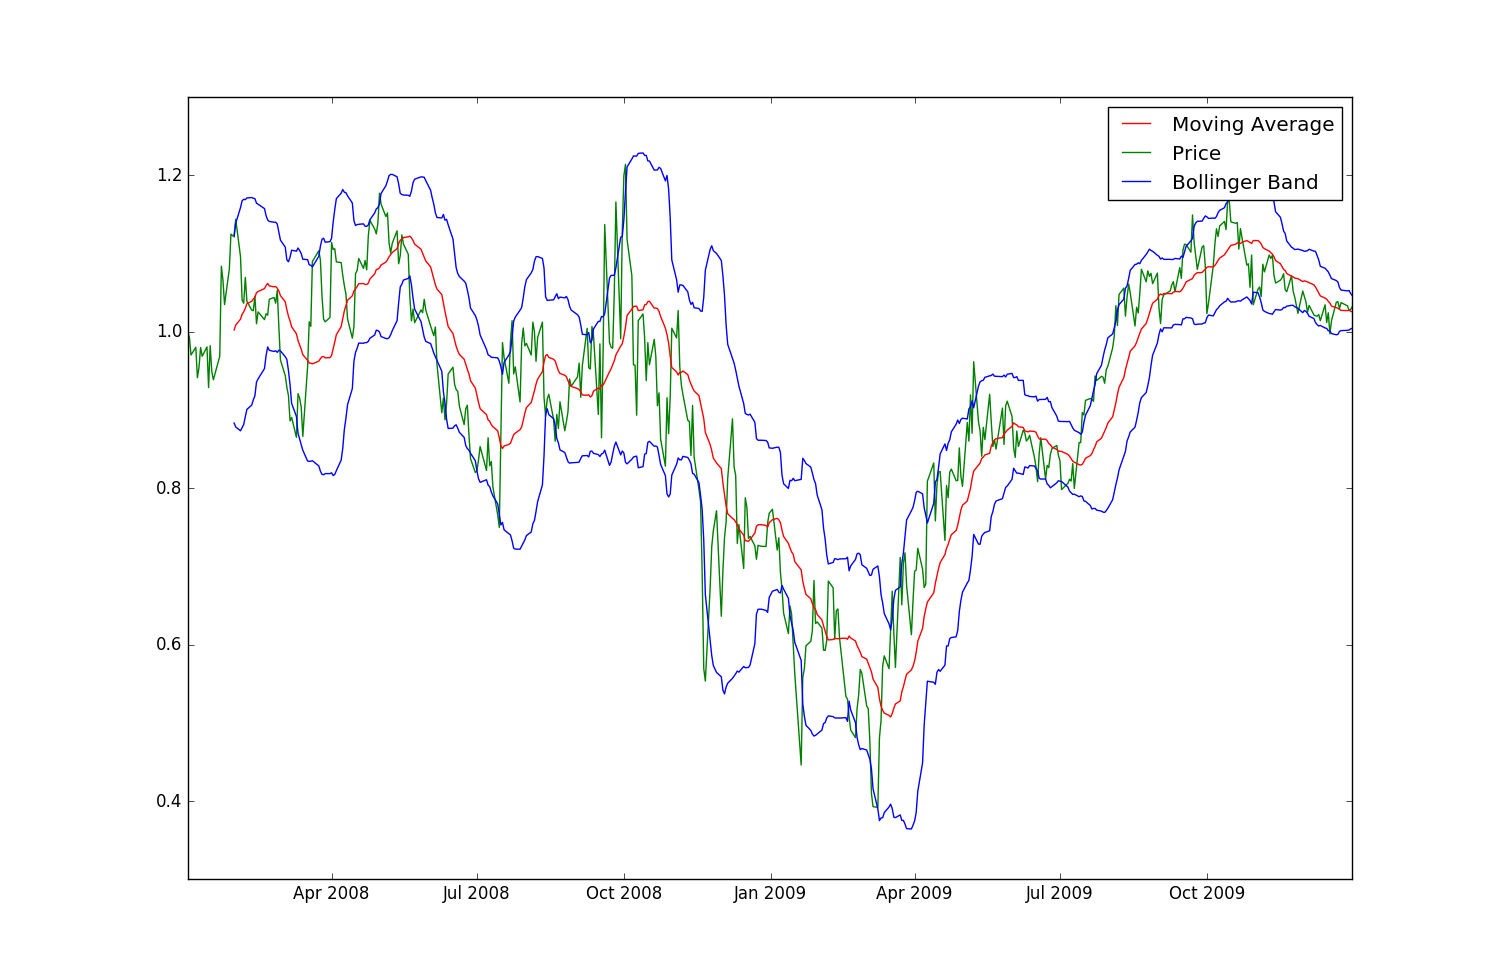
\includegraphics[width=\textwidth]{BB}
		The chart above is created with window size 10. And we can see from the chart that when the price (green line)
		goes outside of the Bollinger Band (blue lines), it typically will bounce back soon, and so the indicator should
		probably work.
\end{itemize}
\subsection{Exponential Moving Average}
	\begin{itemize}
		\item[(a)] Definition \\
				Simple moving average with window size w days at time t can be defined as \\
				$$\alpha = \frac{2}{w + 1}$$

				\[
				   EMA[t]=\left\{
							   \begin{array}{ll}
								 price[0] \text{  if t = 0}\\
								 (1-\alpha)EMA[t-1] + \alpha price[t]  \text{, otherwise}
							   \end{array}
							 \right.
				 \]
				And the indicator of Exponential Moving Average at time t can be defined similarly as indicator of SMA: \\
				\textbf{indicator\_EMA[t] = $\frac{\text{price[t]}}{\text{EMA[t]}} - 1$}
		\item[(b)] Intuition \\
				It is quite similar to the one to SMA, the difference is how you calculate the average,
				and one of the advantage of this is that EMA has values everywhere, whereas
				simple moving average will not have values in the first window. Also, it actually takes
				into account of all the values before, but gradually decays.

		\item[(c)] Chart and Analysis\\
			% 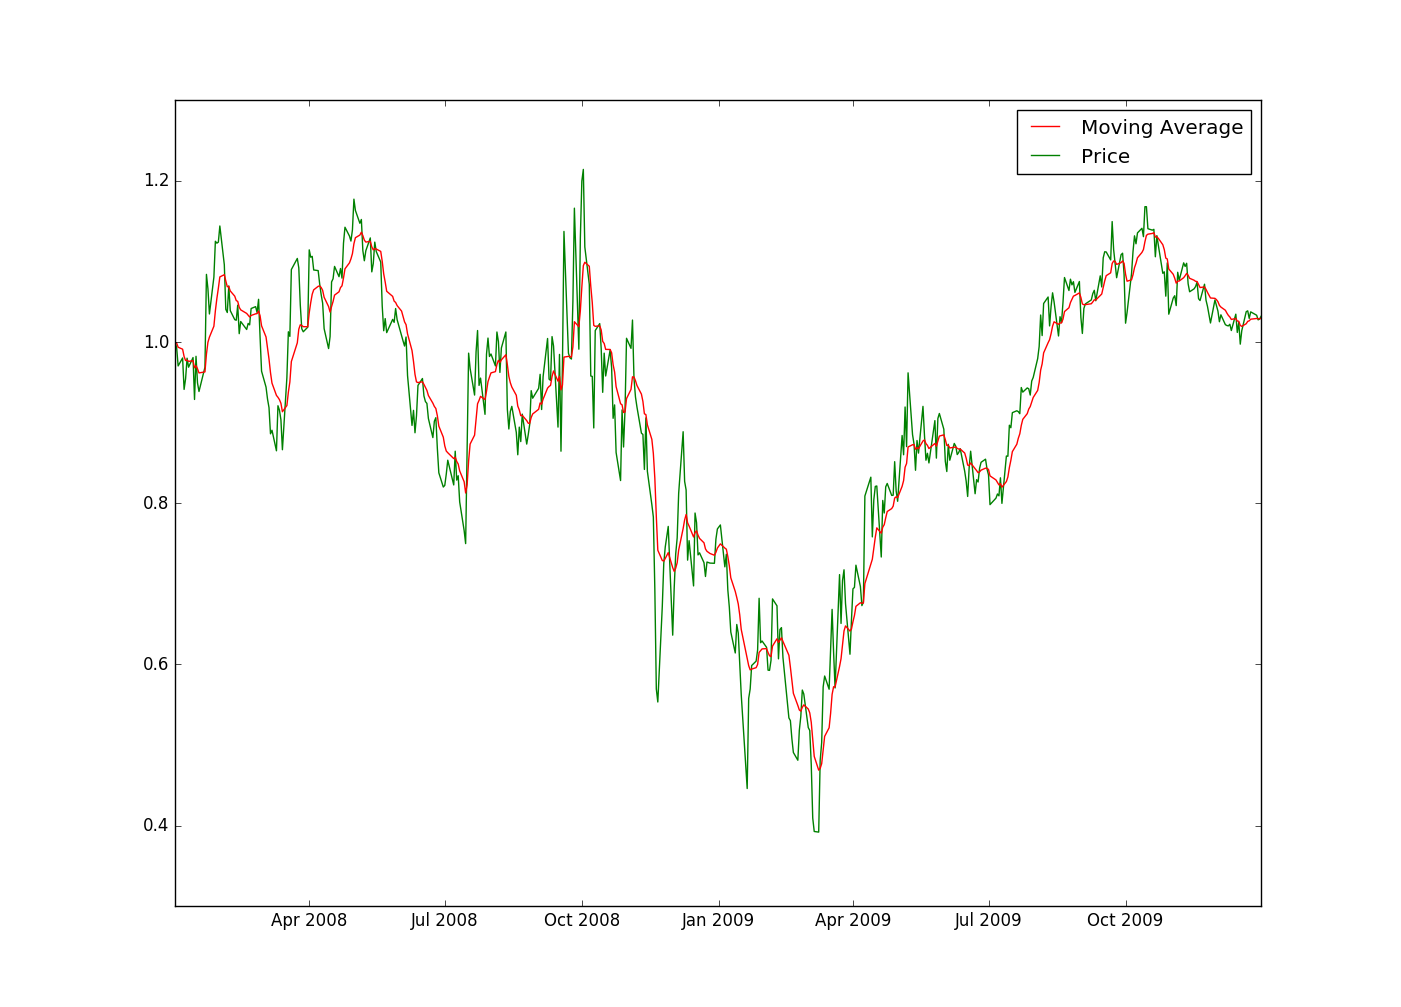
\includegraphics[width=\textwidth]{ema}
			\begin{figure}[!htb]
			\minipage{0.48\textwidth}
			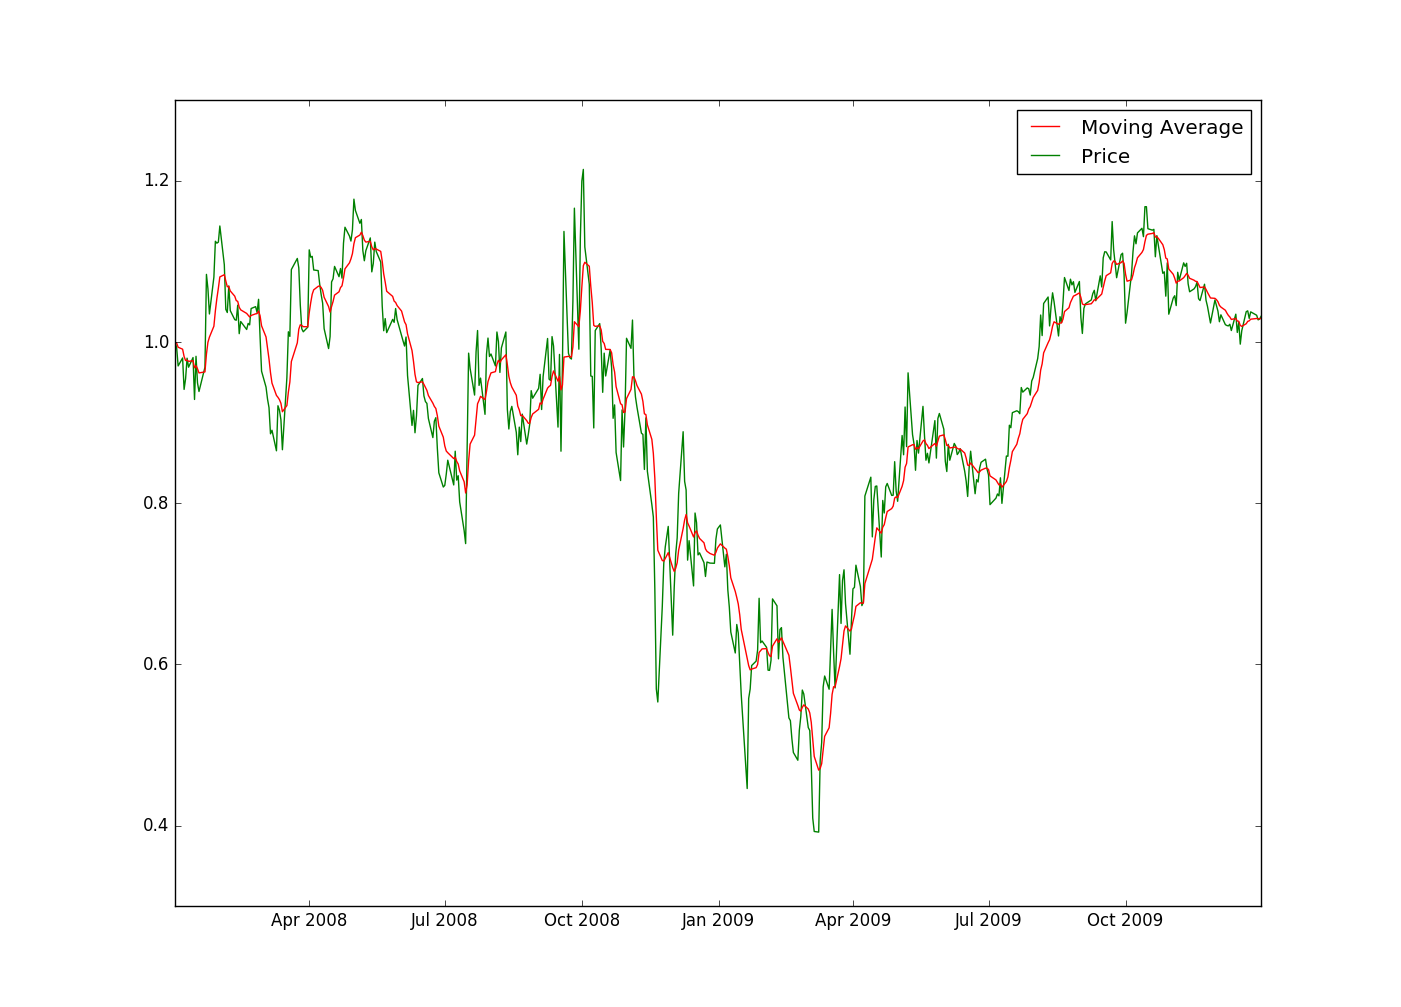
\includegraphics[width=\linewidth]{ema.png}
			\caption{Exponential moving average}\label{fig:awesome_image1}
			\endminipage\hfill
			\minipage{0.48\textwidth}
			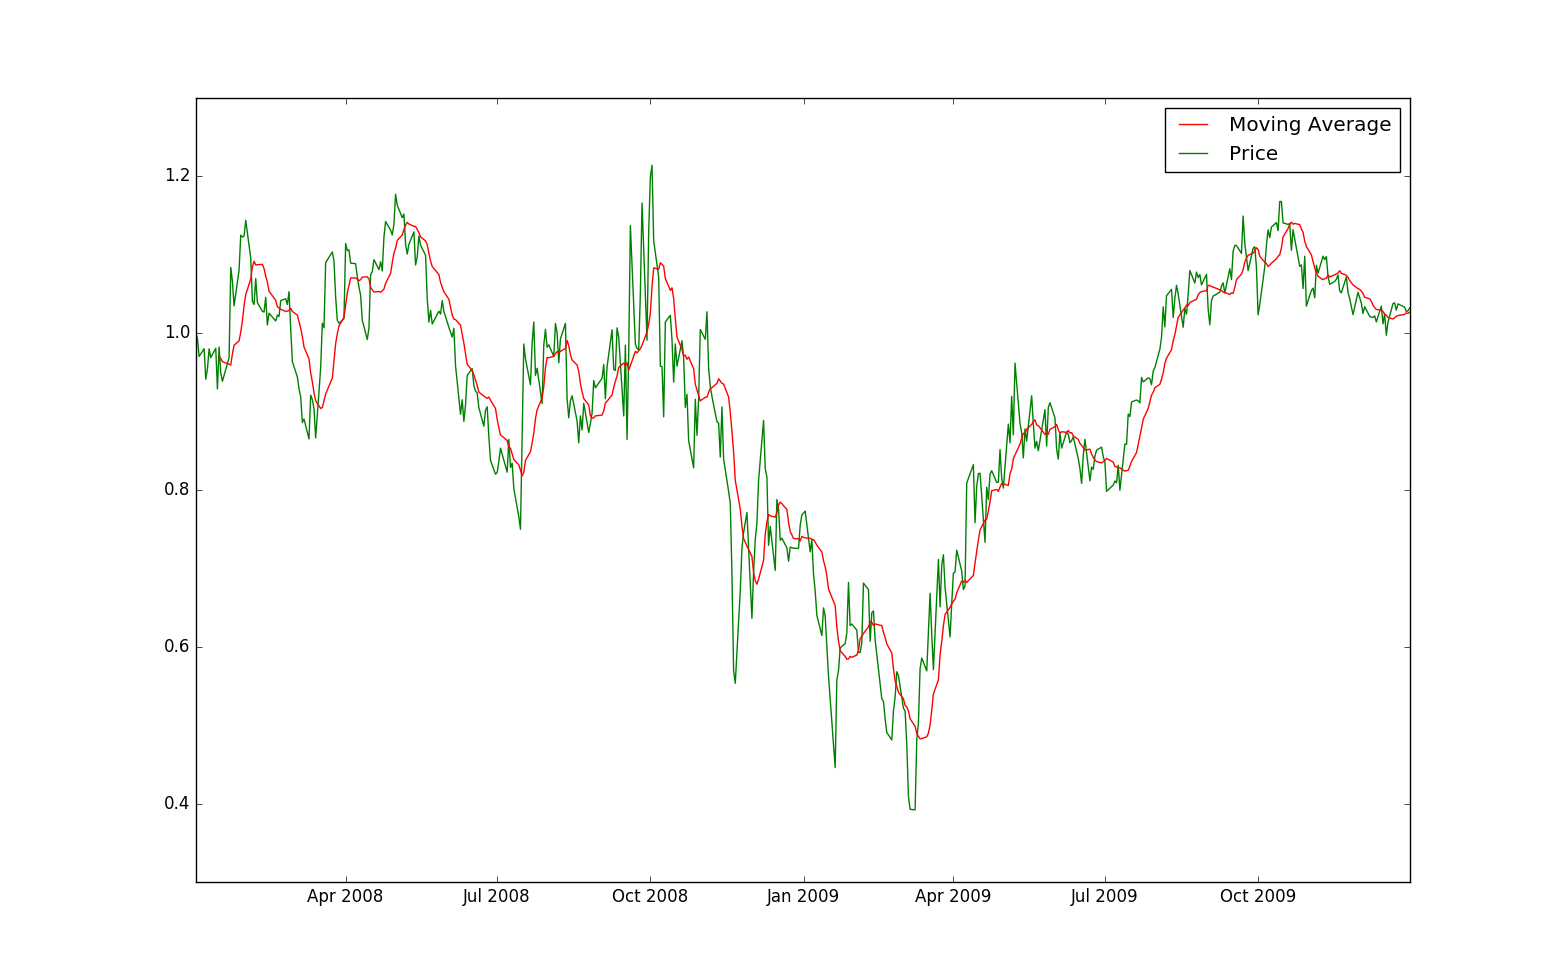
\includegraphics[width=\linewidth]{sma.png}
			\caption{Simple moving average}\label{fig:awesome_image2}
			\endminipage

			\end{figure}
			The charts below look very similar, and they work similarly.
	\end{itemize}


\section{Best Possible Strategy}
\subsection{Assumptions}
	\begin{enumerate}
		\item No transaction fee
		\item No market impact
		\item Allowed to buy at adjusted close only
		\item Only trade for JPM
		\item Stock positions are 1 of 3: short 1000 shares, 0 share, long 1000 shares
		\item No limit on leverage
	\end{enumerate}
\subsection{Algorithm}
	Since we already know the future, so we can always buy at low and sell at high. Also, since there's no
	transaction fee and market impact, we can make as many transactions as we want. Furthermore, we don't need to
	worry about running out of money because we can leverage as much as we can. \\
	So the algorithm combined with above mentioned conditions is very simple, at the first day, we see if the price is
	going down or up, buy 1000 if going up, sell 1000 otherwise. And for the trades afterwards, when hitting local maxima,
	sell 2000 shares, and when hitting local minima, buy 2000 shares, and we can guarantee the holding will be within the
	three positions, and at the same time get the highest yield.
\subsection{Results}

	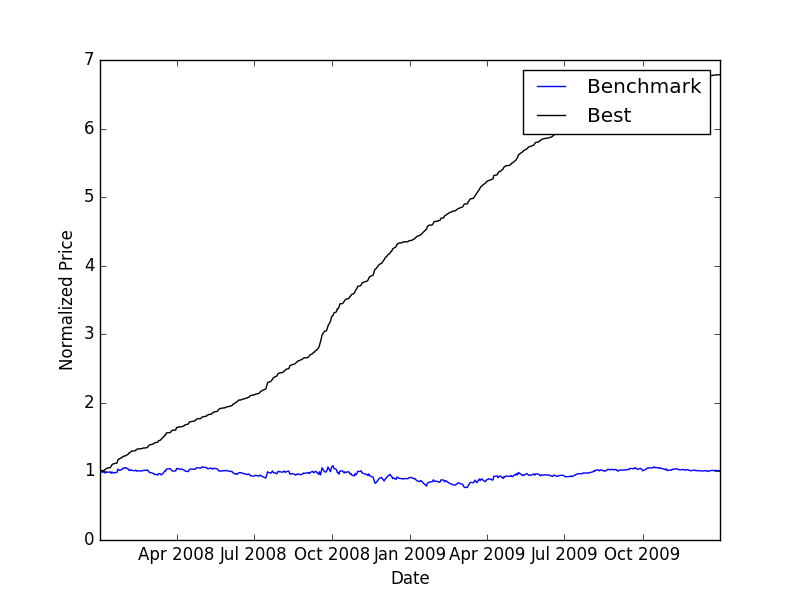
\includegraphics[width=\textwidth]{figure_1}
	Comparison between the two strategies:
	\begin{center}
  	\begin{tabular}{ | l | c | c |}
    \hline
     					& Benchmark & Best Possible Strategy \\ \hline
    Cumulative Return   & 0.0123 & 5.7861 \\ \hline
    Standard Deviation  & 0.0170 & 0.0045 \\ \hline
	Standard Deviation  & 0.0001 & 0.0038 \\ \hline

  \end{tabular}
\end{center}

\section{Manual Strategy}
\subsection{Trading Strategy}
	My strategy is simple, I simply look at the simple moving average indicator,
	if the indicator is smaller than -0.1, I buy as much as I can, and if the indicator
	is bigger than 0.1, I sell as much as I can. Typically, I would like to buy whenever
	the indicator is smaller than 0, and sell whenever the indicator is bigger than 0.
	However, mainly because of the assumption of impact 0.05, we need to do less trades.
	So I only do trades when the absolute values are big enough, and after my tuning, 0.1
	is a good one, with bigger value, it barely does trades, with smaller ones, it does too many.
\subsection{Performance}
	The strategy I proposed has a cumulative return of 9.7\% which is better than 1.7\% benchmark.
	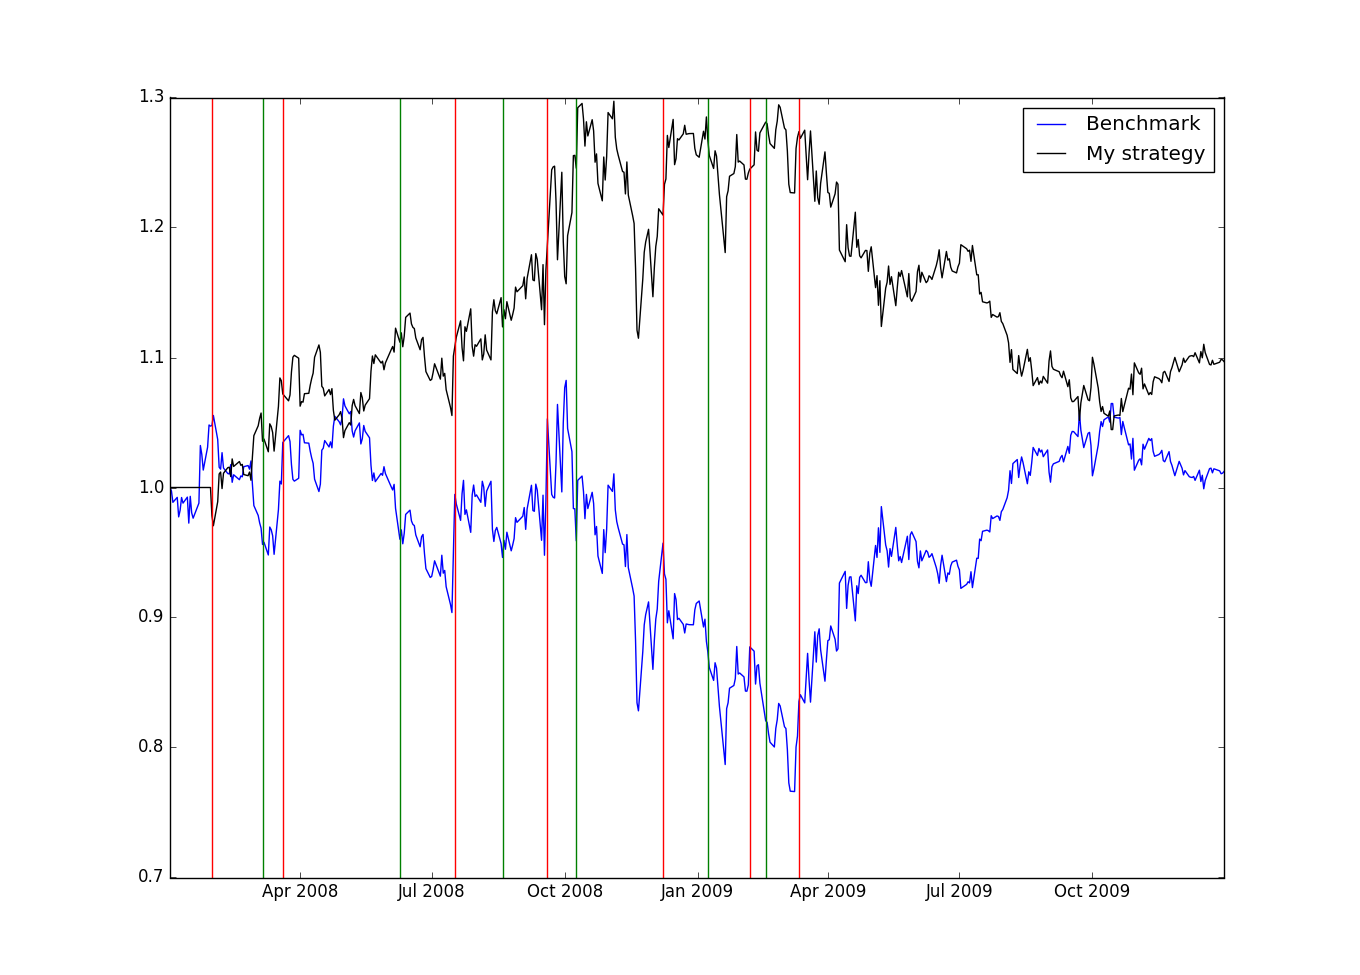
\includegraphics[width=\textwidth]{in_sample_manual}

\section{Comparative Analysis}
\subsection{Results}
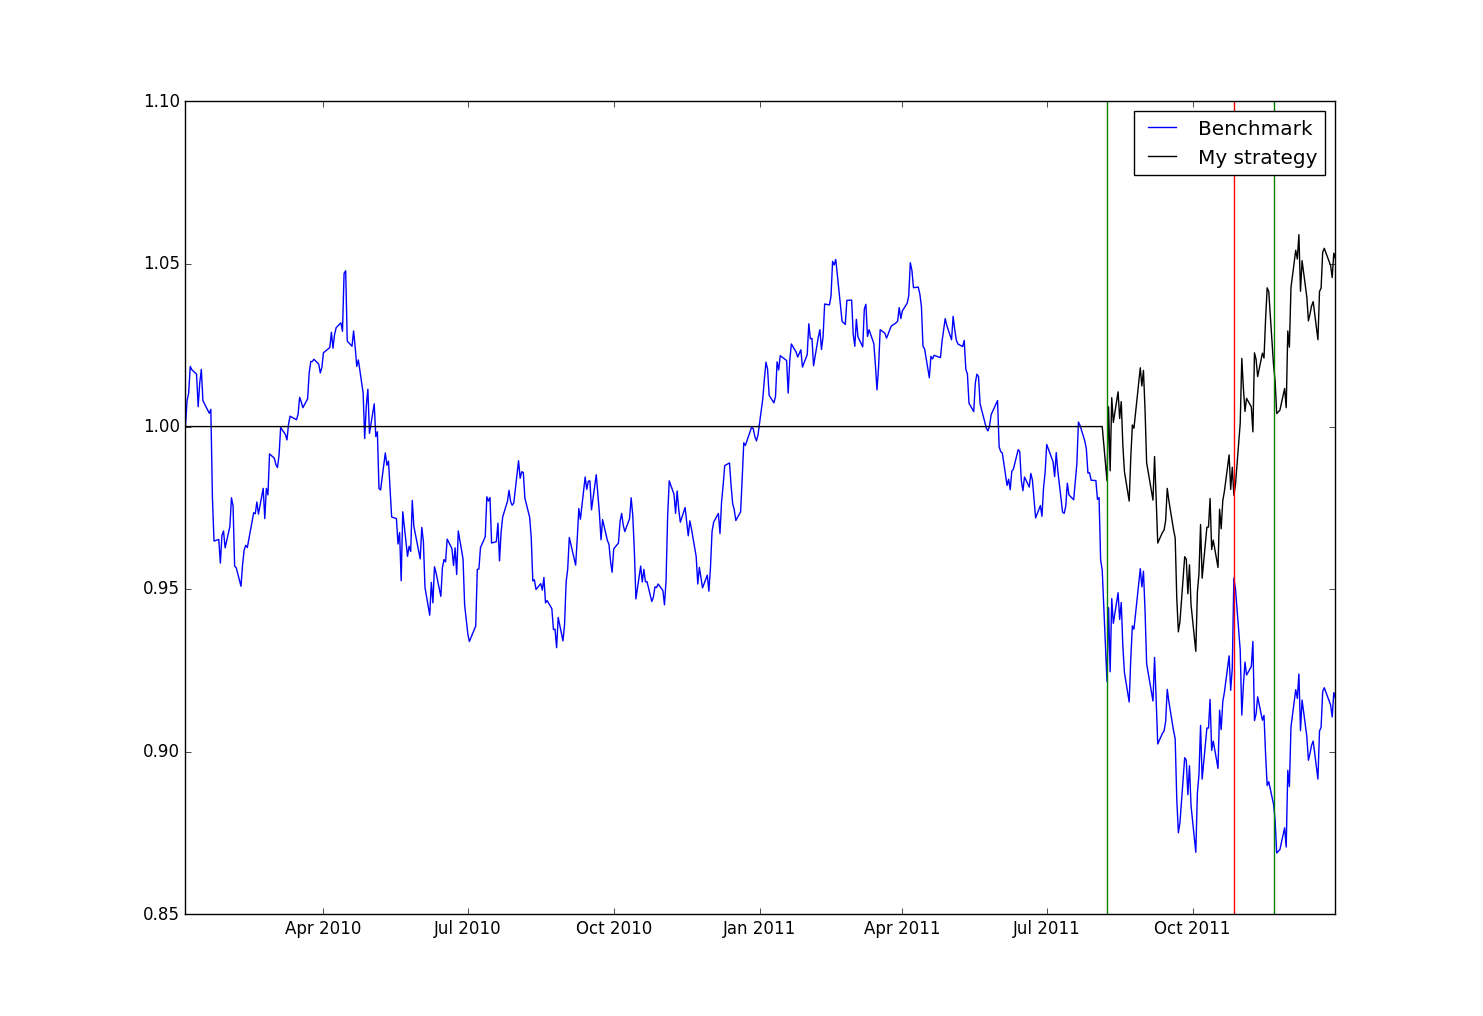
\includegraphics[width=\textwidth]{out_sample_manual}
\begin{center}
\begin{tabular}{ | l | c | c |}
\hline
			                     & Benchmark & Manual \\ \hline
In sample cumulative return      & 0.017     & 0.097 \\ \hline
Out of sample cumulative return  & -0.083    & 0.052 \\ \hline

\end{tabular}
\end{center}
\subsection{Observation and Analysis}
Since we only tune the parameters based on in sample data, the performance betweeen
in sample data and out of sample data can be very different. With the same parameters,
I only trade for three times in the out of sample data, and made 10 in in sample data.
I would say the reason I make money is partly because of my strategy is more conservative.
I don't do trades until there's an obvious enough signal, and by doing this,
I circumvent the situation of paying a lot of 5 percent fee (impact).
\end{document}
